% Options for packages loaded elsewhere
\PassOptionsToPackage{unicode}{hyperref}
\PassOptionsToPackage{hyphens}{url}
\documentclass[
]{article}
\usepackage{xcolor}
\usepackage{amsmath,amssymb}
\setcounter{secnumdepth}{-\maxdimen} % remove section numbering
\usepackage{iftex}
\ifPDFTeX
  \usepackage[T1]{fontenc}
  \usepackage[utf8]{inputenc}
  \usepackage{textcomp} % provide euro and other symbols
\else % if luatex or xetex
  \usepackage{unicode-math} % this also loads fontspec
  \defaultfontfeatures{Scale=MatchLowercase}
  \defaultfontfeatures[\rmfamily]{Ligatures=TeX,Scale=1}
\fi
\usepackage{lmodern}
\ifPDFTeX\else
  % xetex/luatex font selection
\fi
% Use upquote if available, for straight quotes in verbatim environments
\IfFileExists{upquote.sty}{\usepackage{upquote}}{}
\IfFileExists{microtype.sty}{% use microtype if available
  \usepackage[]{microtype}
  \UseMicrotypeSet[protrusion]{basicmath} % disable protrusion for tt fonts
}{}
\makeatletter
\@ifundefined{KOMAClassName}{% if non-KOMA class
  \IfFileExists{parskip.sty}{%
    \usepackage{parskip}
  }{% else
    \setlength{\parindent}{0pt}
    \setlength{\parskip}{6pt plus 2pt minus 1pt}}
}{% if KOMA class
  \KOMAoptions{parskip=half}}
\makeatother
\usepackage{longtable,booktabs,array}
\usepackage{caption}
\captionsetup[table]{skip=6pt}
\newcounter{none} % for unnumbered tables
\usepackage{calc} % for calculating minipage widths
% Correct order of tables after \paragraph or \subparagraph
\usepackage{etoolbox}
\makeatletter
\patchcmd\longtable{\par}{\if@noskipsec\mbox{}\fi\par}{}{}
\makeatother
% Allow footnotes in longtable head/foot
\IfFileExists{footnotehyper.sty}{\usepackage{footnotehyper}}{\usepackage{footnote}}
\makesavenoteenv{longtable}
\usepackage{graphicx}
\makeatletter
\newsavebox\pandoc@box
\newcommand*\pandocbounded[1]{% scales image to fit in text height/width
  \sbox\pandoc@box{#1}%
  \Gscale@div\@tempa{\textheight}{\dimexpr\ht\pandoc@box+\dp\pandoc@box\relax}%
  \Gscale@div\@tempb{\linewidth}{\wd\pandoc@box}%
  \ifdim\@tempb\p@<\@tempa\p@\let\@tempa\@tempb\fi% select the smaller of both
  \ifdim\@tempa\p@<\p@\scalebox{\@tempa}{\usebox\pandoc@box}%
  \else\usebox{\pandoc@box}%
  \fi%
}
% Set default figure placement to htbp
\def\fps@figure{htbp}
\makeatother
\setlength{\emergencystretch}{3em} % prevent overfull lines
\providecommand{\tightlist}{%
  \setlength{\itemsep}{0pt}\setlength{\parskip}{0pt}}
\usepackage{bookmark}
\IfFileExists{xurl.sty}{\usepackage{xurl}}{} % add URL line breaks if available
\urlstyle{same}
% fallback for those not using the hyperref driver hyperxmp:
\makeatletter
\@ifundefined{xmpquote}{\newcommand{\xmpquote}[1]{#1}}{}
\makeatother
\hypersetup{
  hidelinks,
  pdfcreator={LaTeX via pandoc}}

\author{}
\date{}

\begin{document}

{\def\LTcaptype{none} % do not increment counter
\begin{longtable}[]{@{}
  >{\centering\arraybackslash}p{(\linewidth - 2\tabcolsep) * \real{0.1942}}
  >{\raggedright\arraybackslash}p{(\linewidth - 2\tabcolsep) * \real{0.8058}}@{}}
\toprule\noalign{}
\begin{minipage}[b]{\linewidth}\centering

\includegraphics[width=1.19028in,height=1.02569in,alt={Imagine similară}]{images/media/image1.jpeg}
\end{minipage} & \begin{minipage}[b]{\linewidth}\centering
\textbf{Technical University of Moldova}

\textbf{Faculty of Computers, Informatics, and Microelectronics}

\textbf{Department of Software Engineering and Automation}

\textbf{Software Engineering Study Programme}
\end{minipage} \\
\midrule\noalign{}
\endhead
\bottomrule\noalign{}
\endlastfoot
\end{longtable}
}

\textbf{INTERNSHIP REPORT}

\textbf{Project title}

\textbf{Team No. \ldots{}}

\begin{quote}
Team members:
\end{quote}

{\def\LTcaptype{none} % do not increment counter
\begin{longtable}[]{@{}
  >{\raggedright\arraybackslash}p{(\linewidth - 4\tabcolsep) * \real{0.1810}}
  >{\raggedright\arraybackslash}p{(\linewidth - 4\tabcolsep) * \real{0.2923}}
  >{\raggedright\arraybackslash}p{(\linewidth - 4\tabcolsep) * \real{0.1586}}@{}}
\toprule\noalign{}
\begin{minipage}[b]{\linewidth}\raggedright
Student 1:

Student 2:

Student 3. etc.
\end{minipage} & \begin{minipage}[b]{\linewidth}\raggedright
Name Surname, group

Name Surname, group

Name Surname, group
\end{minipage} & \begin{minipage}[b]{\linewidth}\raggedright
*Signature

*Signature

*Signature
\end{minipage} \\
\midrule\noalign{}
\endhead
\bottomrule\noalign{}
\endlastfoot
Mentor: & Name Surname, title & Signature \\
\end{longtable}
}

\textbf{*}By signing the cover page of this report, each student
confirms their active involvement in both the development of the project
and the writing of the report. Students who did not contribute
meaningfully are not permitted to sign.

Submission date: {[}DD/MM/YYYY{]}

\textbf{Chisinau, 2025}

To ensure a clear, well-structured, and professional final paper,
standard formatting rules must be followed. These guidelines help
organize the content in line with academic requirements and make the
thesis easier to read and evaluate. Proper formatting also reflects
precision and responsibility in academic work.

\begin{itemize}
\item
  The report must be written in an impersonal style (the use of
  first-person pronouns is not permitted).
\item
  The main body text shall be formatted as follows: \textbf{Times New
  Roman, 12 pt., 1.5 line spacing, justified alignment, black font
  color}.
\item
  Page margins (without borders or additional inscriptions): \textbf{Top
  -- 20 mm; Bottom -- 20 mm; Left -- 20 mm; Right -- 10 mm}.
\item
  Chapters and subchapters shall be numbered with Arabic numerals (e.g.,
  1, 2, 3; or 1.1, 1.2; or 1.1.1, 1.1.2). Up to three levels are
  accepted. The Introduction and Conclusions are not numbered and should
  not include the word Chapter.
\item
  Source code must be formatted in Courier New, 10 pt., single spacing.
  If the code exceeds 50\% of a page, it must be placed in an appendix,
  with an appropriate reference in the main text.
\item
  Each chapter title must begin on a new page, formatted in uppercase,
  Times New Roman, bold, 13 pt., centered.
\item
  Subchapter titles must be formatted in Times New Roman, bold, 12 pt.,
  left-aligned.
\item
  Chapter and subchapter titles must not appear at the bottom of a page.
\item
  Paragraphs shall be formatted as follows: justified alignment, with
  the first line indented 1.25 cm.
\item
  The spacing between a chapter or subchapter title and the subsequent
  text shall not exceed one line interval.
\item
  A subchapter must cover a minimum of one full page.
\item
  Page numbering shall be placed at the bottom center of each page. The
  title page and preliminary pages before the Introduction are included
  in the total page count but shall not display page numbers.
\item
  The report must be printed on A4 paper, single-sided.
\item
  The text must use clear and precise language, presenting information
  in a direct, intelligible, and logically structured manner. The report
  must reflect the authors' original contribution. All bibliographic
  sources must be cited in-text and listed in the bibliography.
\end{itemize}

{\def\LTcaptype{none} % do not increment counter
\begin{longtable}[]{@{}
  >{\raggedright\arraybackslash}p{(\linewidth - 2\tabcolsep) * \real{0.1685}}
  >{\raggedright\arraybackslash}p{(\linewidth - 2\tabcolsep) * \real{0.8315}}@{}}
\toprule\noalign{}
\begin{minipage}[b]{\linewidth}\raggedright
\textbf{Abstract}
\end{minipage} & \begin{minipage}[b]{\linewidth}\raggedright
A concise summary of your entire report, including:

\begin{itemize}
\item
  the problem addressed
\item
  the proposed solution concept
\item
  main findings and outcomes so far
\item
  objectives, methods, and anticipated impact
\end{itemize}
\end{minipage} \\
\midrule\noalign{}
\endhead
\bottomrule\noalign{}
\endlastfoot
\textbf{Introduction} & \begin{minipage}[t]{\linewidth}\raggedright
\begin{itemize}
\item
  Context and background of the problem
\item
  Motivation and relevance of the project
\item
  Potential impact on the target audience/market
\item
  Brief outline of the report structure
\end{itemize}
\end{minipage} \\
\textbf{Domain Analysis} & \begin{minipage}[t]{\linewidth}\raggedright
\begin{itemize}
\item
  Problem Overview: Define the issue, its significance, and the broader
  context.
\item
  Target Audience: Identify who will use the application, their needs,
  and potential benefits. Use data (interviews, surveys, questionnaires)
  where possible.
\item
  Solution Concept: Describe the application, its purpose, and main
  features.
\item
  Market Research: Compare your idea with existing solutions, identify
  gaps, and explain how your project improves or innovates.
\end{itemize}
\end{minipage} \\
\textbf{System Design} & \begin{minipage}[t]{\linewidth}\raggedright
\begin{itemize}
\item
  \textbf{Technical Requirements}

  \begin{itemize}
  \item
    Functional Requirements: core features and operations.
  \item
    Non-Functional Requirements: performance, usability, and security
    standards.
  \end{itemize}
\item
  \textbf{Behavioral Modeling (UML)}

  \begin{itemize}
  \item
    Use Case Diagrams (system-user interactions).
  \item
    Sequence Diagrams (order of operations).
  \end{itemize}
\item
  \textbf{Structural Modeling (UML)}

  \begin{itemize}
  \item
    Class or Component Diagrams (system architecture and relationships).
  \end{itemize}
\end{itemize}
\end{minipage} \\
\textbf{Conclusions} & \begin{minipage}[t]{\linewidth}\raggedright
\begin{itemize}
\item
  Summary of findings from Domain Analysis and System Design
\item
  Achievements and challenges addressed so far
\item
  Next steps for further development in the PBL course
\item
  Early considerations for implementation
\end{itemize}
\end{minipage} \\
\textbf{Bibliography} & \begin{minipage}[t]{\linewidth}\raggedright
\begin{itemize}
\item
  Include all sources cited in the report (articles, books, research
  papers, websites)
\end{itemize}
\end{minipage} \\
\textbf{Final notes} & \begin{minipage}[t]{\linewidth}\raggedright
\begin{itemize}
\item
  This template is flexible; adapt it to your project needs while
  keeping the \textbf{key sections intact}.
\item
  Students may use the \textbf{LaTeX template provided}, already adapted
  to the required standards. This is optional, but highly recommended
  for those wishing to learn a professional tool for academic writing.
\item
  Total length: \textbf{25--30 pages}.
\end{itemize}
\end{minipage} \\
\end{longtable}
}

\textbf{\hfill\break
}

\textbf{Enumeration in context}

If the text includes simple lists, they are marked with dashes. Each
item begins with a lowercase letter, and each line ends with a
semicolon; a period is placed after the final item.

\emph{Example:}

\begin{itemize}
\item
  \ldots.. one;
\item
  \ldots.. two;
\item
  \ldots.. three.
\end{itemize}

If the list is referenced in the text, enumeration is done using
lowercase Latin letters followed by a closing parenthesis.

If multiple levels of enumeration are needed, lowercase \emph{Latin
letters} followed by a closing parenthesis are used for the first level,
and \emph{Arabic numerals} with a closing parenthesis are used for the
secondary level.

\emph{Example:}

\begin{enumerate}
\def\labelenumi{\alph{enumi})}
\item
  \_\_\_\_\_\_\_\_\_\_\_\_\_\_;
\item
  \_\_\_\_\_\_\_\_\_\_\_\_\_\_;
\end{enumerate}

\begin{enumerate}
\def\labelenumi{\arabic{enumi})}
\item
  \_\_\_\_\_\_\_\_\_\_\_\_\_\_;
\end{enumerate}

\begin{itemize}
\item
  \_\_\_\_\_\_\_\_\_\_\_;
\item
  \_\_\_\_\_\_\_\_\_\_\_;
\end{itemize}

\begin{enumerate}
\def\labelenumi{\arabic{enumi})}
\setcounter{enumi}{1}
\item
  \_\_\_\_\_\_\_\_\_\_\_\_\_\_;
\end{enumerate}

\begin{enumerate}
\def\labelenumi{\alph{enumi})}
\setcounter{enumi}{2}
\item
  \_\_\_\_\_\_\_\_\_\_\_\_\_\_.
\end{enumerate}

Use of any other symbols is prohibited.

\emph{Each item in a list must not exceed one sentence in length.}

\textbf{Figures}

Figures must be numbered sequentially within each chapter: the first
digit indicates the chapter number, and the second digit represents the
order of the figure within that chapter, formatted as ``Figure 1.1''.

Both the word ``Figure 1.1'' and its title should be centered on the
page, written in bold, without a period at the end.

If a figure takes more than 75\% of the page's space, it must be
included in an appendix, with a reference made to it in the main text.

Figures may be formatted in landscape orientation if necessary, provided
they are listed in the Appendix and referenced in the main body of the
thesis.

Every figure should be cited within the text and placed immediately
following its first reference.

\emph{Example:}

According to Figure 1.1...

\textbf{Figure 1.1 -- Figure title}

Figures are numbered sequentially regardless of subchapters. Figure
titles must not be positioned at the bottom of the page.

\textbf{Tables}

Tables are numbered consecutively within each chapter, where the first
number represents the chapter and the second number indicates the
table's sequence in that chapter, for example, ``Table 1.1.''

Table titles are positioned above the tables and aligned to the right.
The content within the tables is formatted using an 11pt font size with
single line spacing.

Tables may be presented in landscape orientation if necessary, provided
they are included in the Appendix and referenced accordingly in the
text.

If a table takes up more than 75\% of a page, it should be placed in an
appendix, with a corresponding reference made in the main text.

Every table must be cited in the text, and the table itself should
appear immediately following its first citation.

\emph{Example:}

As shown in Table 1.1, it is recommended that...

\textbf{Table 1.1 -- Table title}

{\def\LTcaptype{none} % do not increment counter
\begin{longtable}[]{@{}
  >{\centering\arraybackslash}p{(\linewidth - 6\tabcolsep) * \real{0.1638}}
  >{\raggedright\arraybackslash}p{(\linewidth - 6\tabcolsep) * \real{0.1539}}
  >{\raggedright\arraybackslash}p{(\linewidth - 6\tabcolsep) * \real{0.1638}}
  >{\raggedright\arraybackslash}p{(\linewidth - 6\tabcolsep) * \real{0.1638}}@{}}
\toprule\noalign{}
\begin{minipage}[b]{\linewidth}\centering
\textbf{A}
\end{minipage} & \begin{minipage}[b]{\linewidth}\centering
\textbf{B}
\end{minipage} & \begin{minipage}[b]{\linewidth}\centering
\textbf{C}
\end{minipage} & \begin{minipage}[b]{\linewidth}\centering
\textbf{D}
\end{minipage} \\
\midrule\noalign{}
\endhead
\bottomrule\noalign{}
\endlastfoot
123 & 125 & 255411 & 553321 \\
123569 & 2548 & 123355 & 1233 \\
\end{longtable}
}

\textbf{Table continuation}

When a table continues on the next page, the title should be placed on
the right side, followed by the phrase ``Continuation of table 1.1'',
also aligned to the right.

\emph{Example:}

\textbf{Continuation of table 1.1}

{\def\LTcaptype{none} % do not increment counter
\begin{longtable}[]{@{}
  >{\centering\arraybackslash}p{(\linewidth - 6\tabcolsep) * \real{0.2297}}
  >{\raggedright\arraybackslash}p{(\linewidth - 6\tabcolsep) * \real{0.2297}}
  >{\raggedright\arraybackslash}p{(\linewidth - 6\tabcolsep) * \real{0.2298}}
  >{\raggedright\arraybackslash}p{(\linewidth - 6\tabcolsep) * \real{0.2298}}@{}}
\toprule\noalign{}
\begin{minipage}[b]{\linewidth}\centering
\textbf{A}
\end{minipage} & \begin{minipage}[b]{\linewidth}\centering
\textbf{B}
\end{minipage} & \begin{minipage}[b]{\linewidth}\centering
\textbf{C}
\end{minipage} & \begin{minipage}[b]{\linewidth}\centering
\textbf{D}
\end{minipage} \\
\midrule\noalign{}
\endhead
\bottomrule\noalign{}
\endlastfoot
1235555 & 12588 & 25541188 & 55332188 \\
1235696778 & 25488 & 12335588 & 123388 \\
\end{longtable}
}

When a table extends over two or more pages, the column headers must be
repeated at the top of each page.

Table titles should not appear at the bottom of the page.

\textbf{Formulas}

Formulas must be numbered using \emph{Arabic numerals} in ascending
order within each chapter.

The first digit indicates the chapter number, while the second
represents the formula\textquotesingle s sequence within that chapter
(e.g., (1.1), (1.2), etc.). Formulas should be centered on the page,
with the numbering placed at the right margin of the line.

All symbols and coefficients used in a formula must be explained
directly below it, in the same order as they appear in the expression.

Each formula must be referenced in the main text, and it should be
inserted immediately after its first citation.

\emph{Example:}

According to formula (1.1), the following calculation is performed...

\emph{Ax+B=C (1.1)}

\textbf{Appendices}

All appendices must be referenced within the main body of the thesis or
project and listed in sequential order (e.g., Appendix A, Appendix B,
etc.). Each appendix should start on a new page and include a title
centred beneath the heading ``Appendix.''

Figures, tables, and formulas included in the appendices should be
numbered using the corresponding appendix letter, for example: Figure
A1, Table B1, Formula C1.

If an appendix contains only one figure or table, its title may serve as
the title of the appendix itself.

\emph{Example:}

\textbf{Appendix A}

\textbf{Title of the Appendix}

\textbf{Table A.1-Table title}

{\def\LTcaptype{none} % do not increment counter
\begin{longtable}[]{@{}
  >{\centering\arraybackslash}p{(\linewidth - 4\tabcolsep) * \real{0.3059}}
  >{\raggedright\arraybackslash}p{(\linewidth - 4\tabcolsep) * \real{0.3060}}
  >{\raggedright\arraybackslash}p{(\linewidth - 4\tabcolsep) * \real{0.3060}}@{}}
\toprule\noalign{}
\begin{minipage}[b]{\linewidth}\centering
\end{minipage} & \begin{minipage}[b]{\linewidth}\centering
\end{minipage} & \begin{minipage}[b]{\linewidth}\centering
\end{minipage} \\
\midrule\noalign{}
\endhead
\bottomrule\noalign{}
\endlastfoot
& & \\
\end{longtable}
}

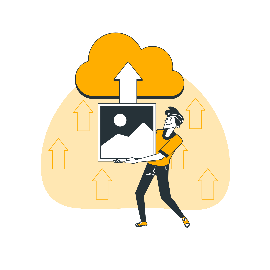
\includegraphics[width=1.04735in,height=1.04735in]{images/media/image2.png}

\textbf{Figure A.1- Figure title}

\textbf{References}

The list of references must follow the order in which the sources are
first cited in the text. Each citation is marked using square brackets:
for example, {[}1{]}, and corresponds to a full entry in the reference
list. This citation style allows the reader to easily identify the
original source of a quoted idea or statement.

Numbers assigned to sources remain consistent throughout the document.
If only a specific section or page is referenced, the page number should
be included in the citation, e.g., {[}8, p. 231{]}.

The bibliography in the thesis must be compiled using the Zotero
application (\url{https://www.zotero.org/}), following the IEEE citation
style.

\end{document}
